%% LyX 2.1.2 created this file.  For more info, see http://www.lyx.org/.
%% Do not edit unless you really know what you are doing.
\documentclass[english]{article}
\usepackage[T1]{fontenc}
\usepackage[latin9]{inputenc}
\usepackage{algorithm2e}
\usepackage{amsmath}
\usepackage{graphicx}
\usepackage{esint}
\usepackage{babel}
\begin{document}

\section{Extra computational challenges}


\subsection{Leak off computation strategies}

To compute $\tau(x)$ it is necessary to find the inverse length function
over the entire interval $x\in(0,1)$. The initial condition gives
a non-zero positive value $l_{*}$ (\ref{initial}), however the information
about the history of the process, including inverse length function,
is not given in the original formulation. It could be understood that
the crack was previously opened and filled with fluid for unknown
time period, or have just been opened and well defined $l^{-1}(x)$
is available. The physical justification for Carter law is that a
cake filter layer is being formed on exposed crack surfaces. Hence
one could expect an impermeable layer to already exist on the initial
opening, or try to use some reference values for early $\tau(x)$
from some known solution. This two approaches will be considered:
\begin{itemize}
\item If the initial fracture was opened for a long time, the initial opening
is fully saturated: 
\begin{equation}
\tau_{a}(x)=\begin{cases}
-\infty & \text{if }0\leq l(t)x\leq l_{*},\\
\tau_{num}(x) & \text{if }l_{*}<l(t)x\leq l(t);
\end{cases}\label{preconditioning_1}
\end{equation}

\item If the initial fracture developed similarly to the zero leak-off self-similar
solution \cite{MWL} (for small time it is reasonable that $\int_{0}^{1}q_{l}(x)dx\rightarrow0$):
\begin{equation}
\tau_{b}(x)=\begin{cases}
\left(x\xi_{*}x_{n}\right)^{5/4}-t_{0}; & \text{if }0\leq l(t)x\leq l_{*},\\
\tau_{num}(x) & \text{if }l_{*}<l(t)x\leq l(t);
\end{cases}\label{preconditioning_2}
\end{equation}

\end{itemize}
(\emph{ewentualnie scenariusz nr 3 pusta szcelina z wybuchu })

where $\tau_{num}(x)$ refers to output of numerical exposure time
calculation scheme (\ref{tau_algorithm}). The effects on $q_{l}$value
of both of these approaches are presented in Figure \ref{leak_tau_a_b}.
The comparison of these two cannot be however completed without understanding
the effect of such on fracture solution. On Figure \ref{different_leak_off_efects}
it is shown how a fracture with sufficiently large leak off can recede
at initial times instead propagating as expected. Further more second
strategy can be extended to two variants

$\tau_{b}^{(1)}$- only recent fracture history is taken into account,
reopened segments are treated as if no cake layer existed

$\tau_{b}^{(2)}$- fracture history is traced form the beginning,
reopened segments are taken into account, thous $\tau_{b}^{(2)}(x)$
might return multiple opening times.

\begin{figure}
\centering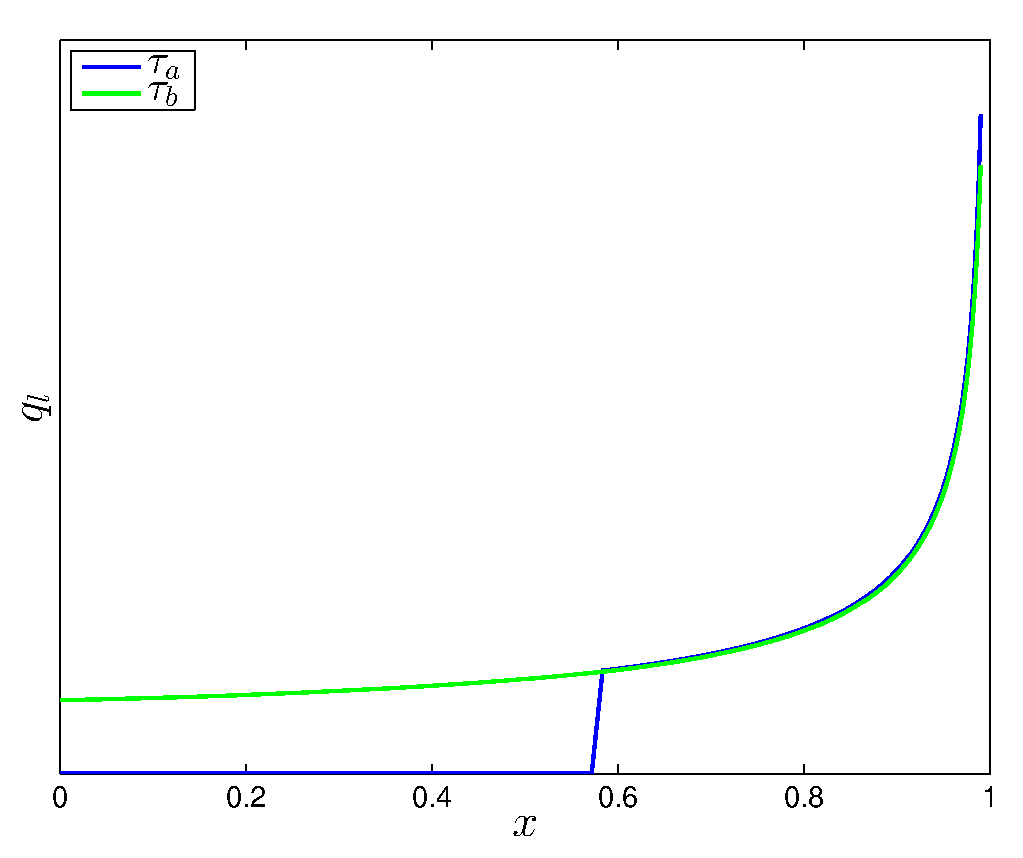
\includegraphics[scale=0.4]{leak_pre_vs_pre}\label{leak_tau_a_b}
\protect\caption{Comparison of leak off variations $\tau_{a}$ and $\tau_{b}$on a
fracure with $l_{*}\approx0.6$}


\end{figure}


\begin{figure}[ht]
\begin{centering}
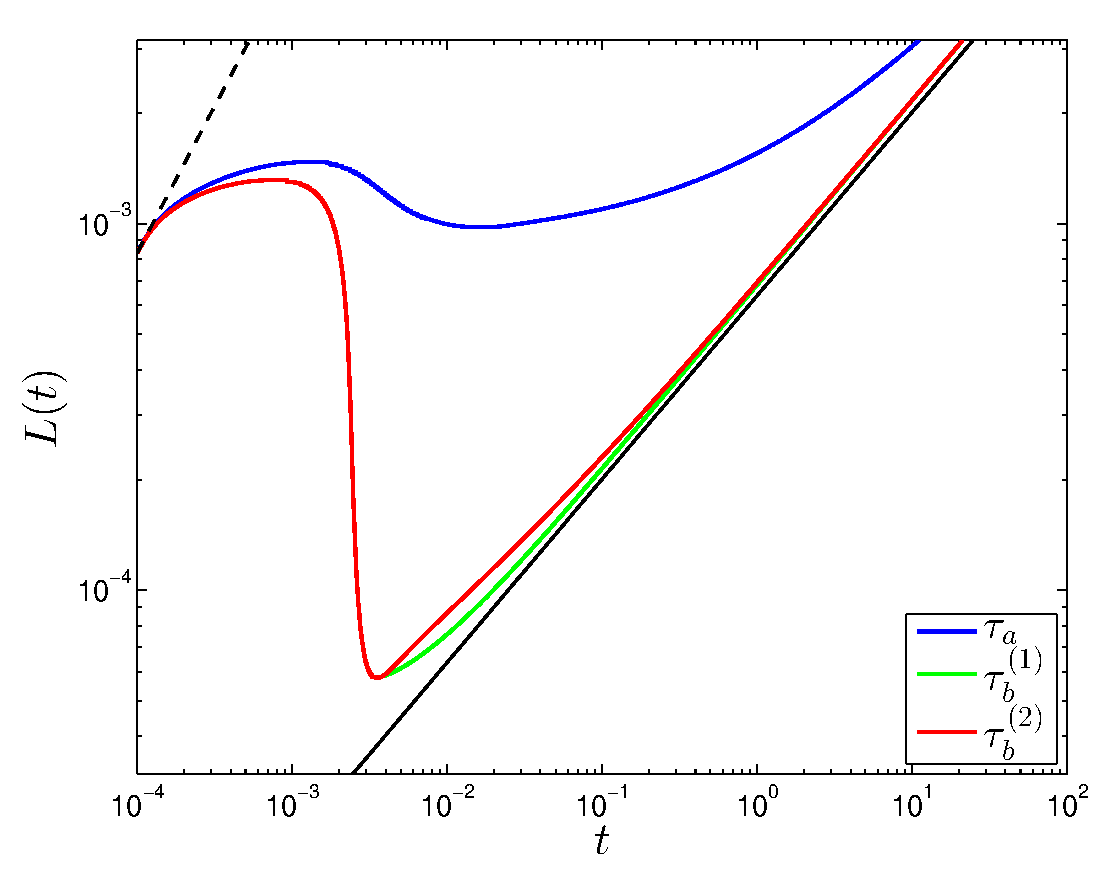
\includegraphics[scale=0.3]{different_leak_off_efects} 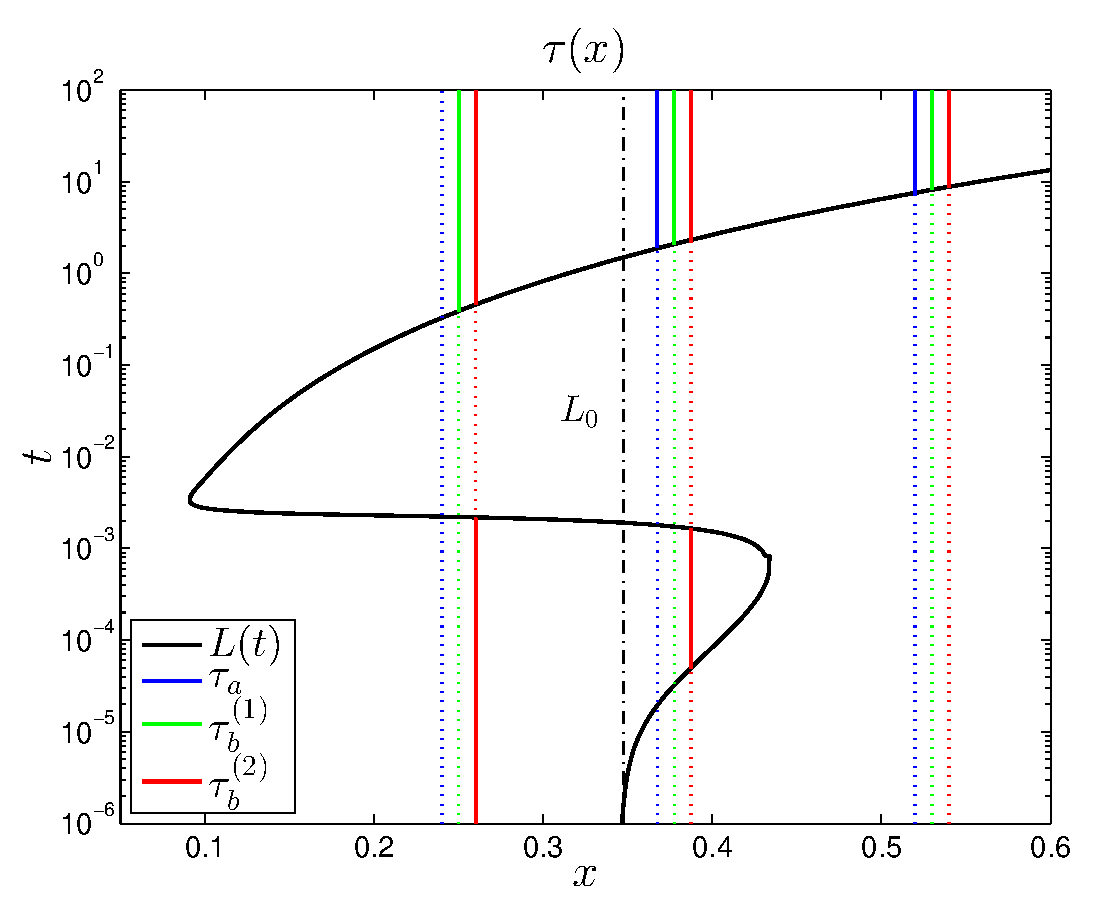
\includegraphics[scale=0.3]{tau_graph} 
\par\end{centering}

\protect\caption{Comparison of effects various interpretations of initial fracture
history and $\tau(x)$ calculation.}


\label{different_leak_off_efects} 
\end{figure}



\subsection{Exposure time computation}

For the both variants of Carter leak-off \ref{carter} it is necessary
to perform additional computation of exposure time $t-\tau(x)$ for
each grid point $x_{i}$. This is however be a separate challenge
on its own, especially if it is to be performed within the derivative
function supplied to an arbitrary ODE solver (as it is in our approach).
Furthermore if a point on was fracture previously opened and closed
several times the exposure time is rather:

\begin{equation}
\tau_{num}(x)=\tau_{1}(x)+\tau_{2}(x)-\tau_{3}(x)+....+\tau_{2N_{\tau}}(x)-\tau_{2N_{\tau}+1}(x)\label{actual_tau}
\end{equation}


Where odd terms are opening times and even times are closure times,
and $N_{\tau}$ is the number of times a fracture was opened. 

As the solution is integrated the function {[}ref{]} is called, and
values of $L(t_{i})$, $t_{i}$, and $V_{0}(t_{i})$ are as calculated
at each call are stored in an sorted, by $t_{i}$, dynamic array.
Values are filtered before insertion so that each value of $L_{i}$
and $t_{i}$ is greater than the previous one, with the exception
of closing fracture events (\ref{frac_closet}). Then when $t-\tau(x)$
is to be found, the formed array is iterated over to form the trajectory
of the crack tip (black line in Figure \ref{different_leak_off_efects}.
As this iteration is made, for each grid point on $x$-axis the number
of times the crack tip passed through that point is accounted for
, as shown by intersections of vertical lines with black line in Figure
\ref{different_leak_off_efects}. Cubic polynomial is interpolated
on two points $(L(t_{i})$, $t_{i})$ , $(L(t_{i+1})$, $t_{i+1})$,
such so $L(t_{i})<xL(t_{i})<L(t_{i+1})$ or $L(t_{i+1})<xL(t_{i})<L(t_{i})$
for closing segments, with derivative conditions from $V_{0}(t_{i})$
and $V_{0}(t_{i+1})$ to approximate this intersections. Finally these
times are combined to obtain total exposure time for each grid point. 

\IncMargin{1em}

\begin{algorithm}
\SetKwData{Left}{left}\SetKwData{This}{this}\SetKwData{Up}{up}
\SetKwFunction{Union}{Union}\SetKwFunction{FindCompress}{FindCompress}
\SetKwInOut{Input}{input}\SetKwInOut{Output}{output}

\Input{vectors with $L(t_{i})$, $t_{i}$ and $V_{0}(t_{i})$, arranged
by their appearance time $t_{i}$, N grid points $x_{k}$} \Output{$\tau_{num}(x_{k})$
as a vector of size N}

\BlankLine

$\tau_{n}(x_{k})-\longleftarrow$ array length $N$ of empty dynamic
arrays length $n$ \; $k\longleftarrow1$\; \For{$i\leftarrow1$
\KwTo length of $t_{i}-1$}{ \If{$L(t_{i+1})\geq L(t_{i})$}{
\Repeat{$x_{k}>L(t_{i})$} { $\tau_{n+1}(x_{k})\longleftarrow$
output of interpolating $L(t),V_{0}(t)$ at $t_{i},t_{i+1}$\; $k\longleftarrow k+1$\;
}

}{

} \If{$L(t_{i+1})<L(t_{i})$}{ \Repeat{$x_{k}<L(t_{i})$}
{ $\tau_{n+1}(x_{k})\longleftarrow$ output of interpolating $L(t),V_{0}(t)$
at $t_{i},t_{i+1}$\; $k:=k-1$\; }

}

}

\For{$i\leftarrow1$ \KwTo $N$}{ $\tau_{num}(x_{k})\longleftarrow\tau_{1}(x_{k})$\;
\For{$j\leftarrow2$ \KwTo length of $\tau_{n}(x_{k})$ }{

\uIf{j even}{ $\tau_{num}(x_{k})\longleftarrow\tau_{num}(x_{k})+\tau_{j}(x_{k})$\;
} \uElse{$\tau_{num}(x_{k})\longleftarrow\tau_{num}(x_{k})-\tau_{j}(x_{k})$\;}

}

}

\label{tau_algorithm}

\protect\caption{Scheme for numerically aproximating $\tau(x)$ in a propagating or
closing fracture}
\end{algorithm}


\DecMargin{1em}


\subsection{Modified closing fracture algorithm}

The original problem formulation was designed strictly for propagating
or already opened fracture. The underlying assumptions were that the
crack propagation speed is positive ($V(1)>0$) and the crack width
is greater than zero ($w(t,x)>0$), except for the crack tip where
$w(t,1)=0$. These could however become invalid under specific conditions.
Fracture remains open as long as fluid flow inside the fracture is
greater than the leak-off, then proposed a simple observation that:
\textit{if the fracture width is monotonically decreasing from mouth
to tip, and the value of leak-off monotonically increases up to the
crack tip, then the first possible non-tip point $x$ where $w(t,x)=0$
is $1-\varepsilon$ for an infinitely small $\varepsilon$}. (pisac
do tego dowod ? dla p carter trzeba porownac $w=()^{1/3}+()^{5/6}$
do $\frac{w}{\sqrt{1-x}}$) 

Noting that MATLAB ODE15s solver provides an option to include events,
lets supply a simple event function:

\begin{equation}
f_{event}(t)=w_{N}.\label{frac_closet}
\end{equation}


Then when the value of the crack width at the last grid point reaches
$w_{N}=0$, ODE15s is going to stop computation. Now it is possible
to restart the computation after a small modification of the solution
at the time the event occurred:

\begin{equation}
l_{*}=(1-\varepsilon)l_{end},\quad\quad w_{*}(x)=w_{end}(x(1-\varepsilon)),\label{event_re-mesh}
\end{equation}


where $l_{end}$ and $w_{end}$ refer to the values at the last time
step. The discretised value $w_{end}$ needs to be extrapolated, this
is done using spline interpolation and asymptotic terms $w_{0}$ and
$w_{1}$ for \textquotedbl{}good enough\textquotedbl{} accuracy. The
fluid balance is satisfied (see subsection ~\ref{subsec:fluid_balance}).
This operation essentially chops off closed fracture segment off the
length $\varepsilon l$, thus it is a discontinuous step, however
the change is relatively small and insignificant. Final solution is
obtained by combining all the outputs together. If fracture is to
decrease significantly, this operation needs to be repeated multiple
times, which might lead to high computational cost, as each backward
step is of order $\varepsilon$. For this reason to compute possibly
closing fractures it would be unwise to use $\varepsilon<10^{-2}$
for closing fracture, but it is possible to use small $\varepsilon$
when fracture is propagating, and switch to a larger value if a change
of propagation regime is detected. Note that this approach should
not be treated as a proper solution to closing fracture problem, it
is a straightforward simplified extension to our propagating fracture
model. Behavior of closing fracture is presented in Figure \ref{closing_zoom}.

\begin{figure}[ht]
\begin{centering}
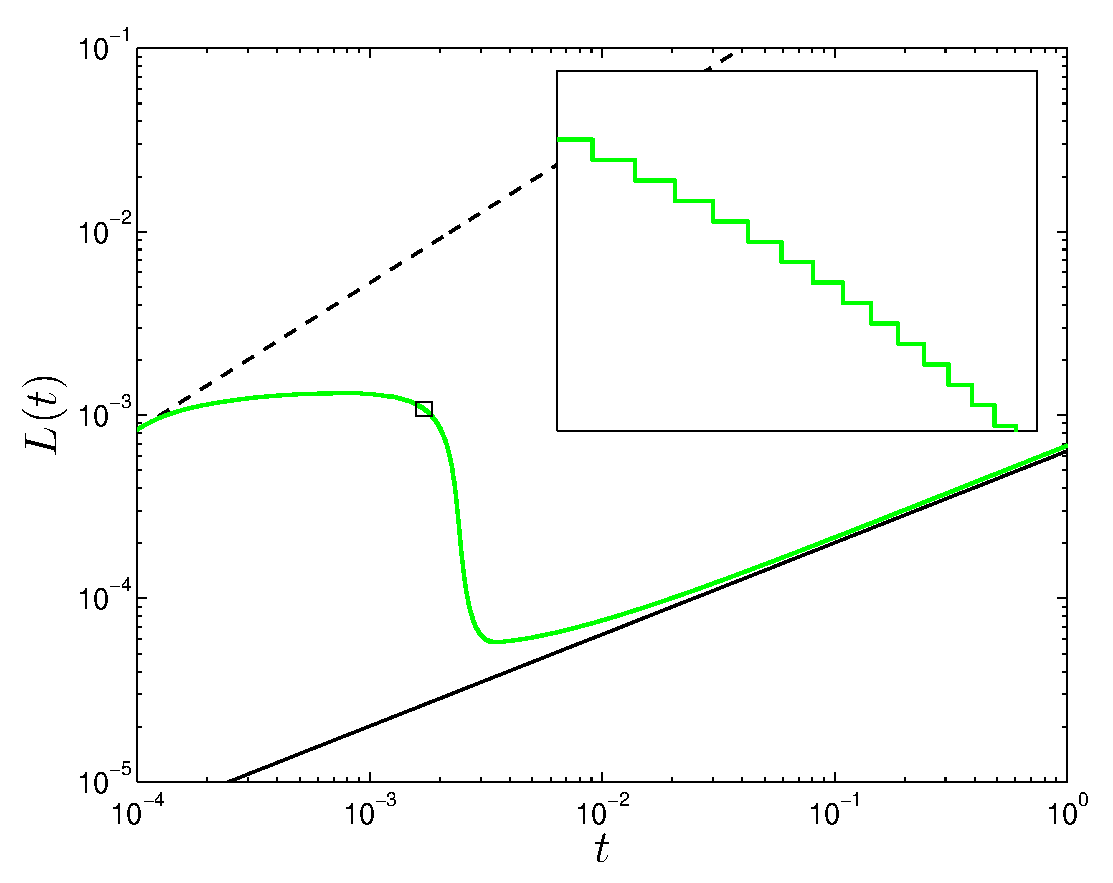
\includegraphics[scale=0.38]{closing-zoom} 
\par\end{centering}

\protect\caption{Close view on closing fracture length. Fracture is allowed to close
by $\varepsilon$ of its length, thus staircase pattern is formed.}


\label{closing_zoom} 
\end{figure}



\subsection{Fluid balance check}

\label{subsec:fluid_balance}

Fluid balance equation is used to verify if solver output is valid:

\begin{equation}
\int_{0}^{t}q_{0}(t)dt=\int_{0}^{1}w_{*}(x)dx+\int_{0}^{t}\int_{0}^{1}w(t,x)dxdt+\int_{0}^{t}\int_{0}^{1}q_{l}(t,x)dxdt.\label{fluid_balance}
\end{equation}


A good way to integrate leak off function$\int_{0}^{t}\int_{0}^{1}q_{l}(t,x)dxdt$
is to add an extra ode to ODE15s, lets call it:

\begin{equation}
\mathcal{\mathcal{C}=}\int_{0}^{1}q_{l}(t,x)dx\label{operator_leak}
\end{equation}


So then the derivative function can be extended by attaching $\mathcal{C}$:

\begin{equation}
\frac{dy}{dt}=\{\mathcal{A},\mathcal{B},\mathcal{\mathcal{C}}\}\label{fluid_balance-2}
\end{equation}

\end{document}
